\documentclass{article}

% content/resources/templates/preamble.tex
\usepackage[margin=0.6in]{geometry}
\author{Milav Dabgar}
\usepackage{amsmath,amssymb,amsthm}
\usepackage{booktabs}
\usepackage{multirow}
\usepackage{xcolor}
\usepackage{tcolorbox}
\tcbuselibrary{breakable,skins}
\usepackage[colorlinks=true,linkcolor=blue]{hyperref}
\usepackage{titlesec}
\usepackage{enumitem}
\usepackage{tikz}
\usepackage{pgfplots}
\usepackage{circuitikz}
\usepackage[version=4]{mhchem}
\usepackage{longtable}
\usepackage{array}
\usepackage{float}
\usepackage{caption}
\usepackage{listings}

\lstset{
  basicstyle=\small\ttfamily,
  breaklines=true,
  breakatwhitespace=false,
  postbreak=\mbox{\textcolor{red}{$\hookrightarrow$}\space},
  float=false,
  numbers=left,
  numberstyle=\tiny\color{gray},
  numbersep=10pt,
  xleftmargin=2em,
  keywordstyle=\color{blue},
  commentstyle=\color{green!60!black},
  stringstyle=\color{purple},
  backgroundcolor=\color{gray!5},
  showstringspaces=false,
  tabsize=2,
  captionpos=b,
  keepspaces=true,
  columns=flexible
}

\pgfplotsset{compat=1.18}
\usetikzlibrary{shapes,arrows,positioning,calc,patterns,decorations.pathmorphing,decorations.markings,arrows.meta}

% Color scheme
\definecolor{headcolor}{RGB}{0,102,204}
\definecolor{keycolor}{RGB}{220,20,60}
\definecolor{solutioncolor}{RGB}{34,139,34}
\definecolor{mnemoniccolor}{RGB}{148,0,211}
\definecolor{codecolor}{RGB}{0,0,100}

% Spacing
\setlength{\parskip}{3pt}
\setlist[itemize]{nosep}
\setlist[enumerate]{nosep}

% Title formatting
\titleformat{\section}{\Large\bfseries\color{headcolor}}{\thesection}{1em}{}
\titleformat{\subsection}{\large\bfseries\color{headcolor}}{\thesubsection}{1em}{}

% Pandoc tightlist compatibility
\providecommand{\tightlist}{%
  \setlength{\itemsep}{0pt}\setlength{\parskip}{0pt}}

% Pandoc longtable compatibility
\newcounter{none}
\def\thenone{}


% content/resources/templates/english-boxes.tex

% Custom environments
\newtcolorbox{solutionbox}{
 breakable,
 enhanced,
 colback=solutioncolor!5!white,
 colframe=solutioncolor!75!black,
 fonttitle=\bfseries,
 title=Solution
}

\newtcolorbox{solutionboxnobreak}{
 colback=solutioncolor!5!white,
 colframe=solutioncolor!75!black,
 fonttitle=\bfseries,
 title=Solution
}

\newtcolorbox{keyformula}{
 breakable,
 enhanced,
 colback=keycolor!5!white,
 colframe=keycolor!75!black,
 fonttitle=\bfseries,
 title=Key Formula
}

\newtcolorbox{mnemonicboxenv}{
 breakable,
 enhanced,
 colback=mnemoniccolor!5!white,
 colframe=mnemoniccolor!75!black,
 fonttitle=\bfseries,
 title=Mnemonic
}

\newcommand{\mnemonicbox}[1]{%
  \begin{mnemonicboxenv}
    #1
  \end{mnemonicboxenv}
}


% Custom commands for GTU solutions
% This file defines semantic commands for consistent formatting

% Question command with automatic formatting
\newcommand{\question}[2]{%
  \section*{Question #1}%
  \textbf{#2}%
}

% OR question variant
\newcommand{\questionor}[2]{%
  \section*{Question #1 OR}%
  \textbf{#2}%
}

% Proper table environment with caption
\newenvironment{answertable}[1]{%
  \begin{table}[htbp]
  \centering
  \caption{#1}
}{%
  \end{table}
}

% Proper figure environment for diagrams
\newenvironment{answerdiagram}[1]{%
  \begin{figure}[htbp]
  \centering
  \caption{#1}
}{%
  \end{figure}
}

% Semantic markup for key terms
\newcommand{\keyword}[1]{\textbf{#1}}
\newcommand{\code}[1]{\texttt{#1}}
\newcommand{\classname}[1]{\texttt{#1}}
\newcommand{\methodname}[1]{\texttt{#1}}

% Proper quotation marks
\newcommand{\mnemonic}[1]{``#1''}


\title{Advanced Java Programming (4351603) - Winter 2023 Solution}
\date{December 8, 2023}

\begin{document}
\maketitle

\questionmarks{1(a)}{3}{Draw and explain swing class hierarchy.}

\begin{solutionbox}
\begin{center}
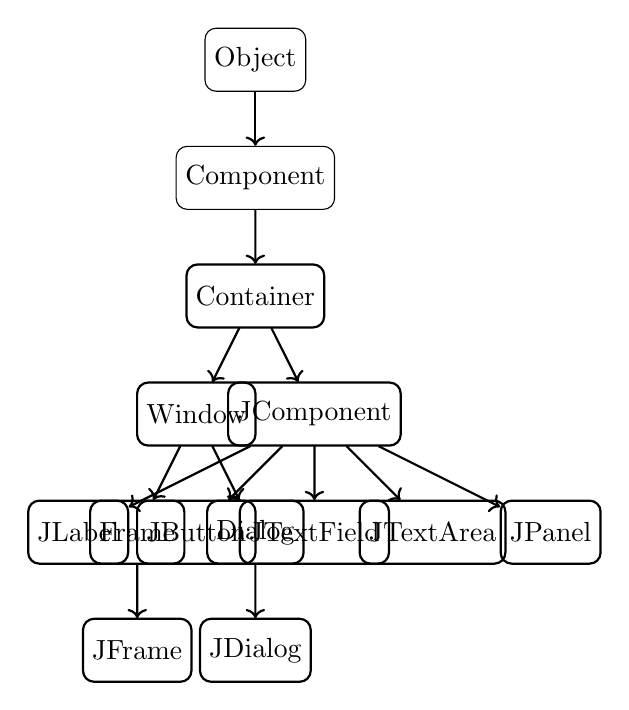
\begin{tikzpicture}[node distance=1.5cm, auto,
    every node/.style={rectangle, draw, rounded corners, minimum height=0.8cm, align=center},
    edge from parent/.style={draw, ->, thick}]
    
    \node {Object}
        child { node {Component}
            child { node {Container}
                child { node {Window}
                    child { node {Frame}
                        child { node {JFrame} }
                    }
                    child { node {Dialog}
                        child { node {JDialog} }
                    }
                }
                child { node {JComponent}
                    child { node {JLabel} }
                    child { node {JButton} }
                    child { node {JTextField} }
                    child { node {JTextArea} }
                    child { node {JPanel} }
                }
            }
        };
\end{tikzpicture}
\captionof{figure}{Swing Class Hierarchy}
\end{center}

\begin{itemize}
    \item \textbf{Component}: Base class for all GUI components.
    \item \textbf{Container}: Components that can hold other components.
    \item \textbf{JComponent}: Base class for all Swing components.
\end{itemize}
\end{solutionbox}

\begin{mnemonicbox}
\mnemonic{Objects Contain Components Jointly}
\end{mnemonicbox}

\questionmarks{1(b)}{4}{List out various Layout Managers. Explain Flow Layout manager with Example.}

\begin{solutionbox}
\begin{center}
\captionof{table}{Layout Managers}
\begin{tabulary}{\linewidth}{|L|L|}
\hline
\textbf{Layout Manager} & \textbf{Description} \\ \hline
\keyword{FlowLayout} & Arranges components left to right \\ \hline
\keyword{BorderLayout} & Five regions: North, South, East, West, Center \\ \hline
\keyword{GridLayout} & Equal-sized rectangular grid \\ \hline
\keyword{CardLayout} & Stack of components \\ \hline
\keyword{BoxLayout} & Single row or column \\ \hline
\end{tabulary}
\end{center}

\textbf{FlowLayout Example:}
\begin{lstlisting}[language=Java]
JFrame frame = new JFrame();
frame.setLayout(new FlowLayout());
frame.add(new JButton("Button1"));
frame.add(new JButton("Button2"));
frame.setSize(300, 100);
frame.setVisible(true);
\end{lstlisting}

\begin{itemize}
    \item \textbf{Default alignment}: Components flow left to right.
    \item \textbf{Wrapping}: Components wrap to next line when needed.
\end{itemize}
\end{solutionbox}

\begin{mnemonicbox}
\mnemonic{Flow Goes Left Right}
\end{mnemonicbox}

\questionmarks{1(c)}{7}{Develop a Java Swing program for a counter application having "Increment" and "Decrement" buttons with initial count of 0 displayed in the label. When "Increment" is clicked, the count increases by 1, and when "Decrement" is clicked, the count decreases by 1. A message dialog should be displayed when the counter goes below 0.}

\begin{solutionbox}
\begin{lstlisting}[language=Java]
import javax.swing.*;
import java.awt.*;
import java.awt.event.*;

public class CounterApp extends JFrame implements ActionListener {
    private int count = 0;
    private JLabel countLabel;
    private JButton incButton, decButton;
    
    public CounterApp() {
        setTitle("Counter Application");
        setLayout(new FlowLayout());
        
        countLabel = new JLabel("Count: " + count);
        incButton = new JButton("Increment");
        decButton = new JButton("Decrement");
        
        incButton.addActionListener(this);
        decButton.addActionListener(this);
        
        add(countLabel);
        add(incButton);
        add(decButton);
        
        setSize(250, 100);
        setDefaultCloseOperation(JFrame.EXIT_ON_CLOSE);
        setVisible(true);
    }
    
    public void actionPerformed(ActionEvent e) {
        if(e.getSource() == incButton) {
            count++;
        } else if(e.getSource() == decButton) {
            count--;
            if(count < 0) {
                JOptionPane.showMessageDialog(this, "Counter below zero!");
            }
        }
        countLabel.setText("Count: " + count);
    }
    
    public static void main(String[] args) {
        new CounterApp();
    }
}
\end{lstlisting}

\begin{itemize}
    \item \textbf{Event handling}: ActionListener interface implementation.
    \item \textbf{Dialog display}: JOptionPane for negative counter warning.
    \item \textbf{Label update}: Real-time count display.
\end{itemize}
\end{solutionbox}

\begin{mnemonicbox}
\mnemonic{Increment Decrements Create Dialogs}
\end{mnemonicbox}

\questionmarks{1(c OR)}{7}{Create a Swing application with a menu bar containing a "File" menu having menu items "New", "Open", and "Exit". When the user clicks "Exit", the application should close. Add keyboard shortcuts for file menu items. Also add a "Help" menu having menu item "About". Display a message box which shows description of this program when `About' is clicked.}

\begin{solutionbox}
\begin{lstlisting}[language=Java]
import javax.swing.*;
import java.awt.event.*;

public class MenuApp extends JFrame implements ActionListener {
    
    public MenuApp() {
        setTitle("Menu Application");
        
        JMenuBar menuBar = new JMenuBar();
        
        JMenu fileMenu = new JMenu("File");
        JMenuItem newItem = new JMenuItem("New");
        JMenuItem openItem = new JMenuItem("Open");
        JMenuItem exitItem = new JMenuItem("Exit");
        
        newItem.setAccelerator(KeyStroke.getKeyStroke(KeyEvent.VK_N, ActionEvent.CTRL_MASK));
        openItem.setAccelerator(KeyStroke.getKeyStroke(KeyEvent.VK_O, ActionEvent.CTRL_MASK));
        exitItem.setAccelerator(KeyStroke.getKeyStroke(KeyEvent.VK_X, ActionEvent.CTRL_MASK));
        
        newItem.addActionListener(this);
        openItem.addActionListener(this);
        exitItem.addActionListener(this);
        
        fileMenu.add(newItem);
        fileMenu.add(openItem);
        fileMenu.addSeparator();
        fileMenu.add(exitItem);
        
        JMenu helpMenu = new JMenu("Help");
        JMenuItem aboutItem = new JMenuItem("About");
        aboutItem.addActionListener(this);
        helpMenu.add(aboutItem);
        
        menuBar.add(fileMenu);
        menuBar.add(helpMenu);
        
        setJMenuBar(menuBar);
        setSize(400, 300);
        setDefaultCloseOperation(JFrame.EXIT_ON_CLOSE);
        setVisible(true);
    }
    
    public void actionPerformed(ActionEvent e) {
        String command = e.getActionCommand();
        
        if(command.equals("Exit")) {
            System.exit(0);
        } else if(command.equals("About")) {
            JOptionPane.showMessageDialog(this, 
                "Menu Application v1.0\nDemonstrates Swing menus with shortcuts");
        }
    }
    
    public static void main(String[] args) {
        new MenuApp();
    }
}
\end{lstlisting}

\begin{itemize}
    \item \textbf{Keyboard shortcuts}: Ctrl+N, Ctrl+O, Ctrl+X accelerators.
    \item \textbf{Menu structure}: File and Help menus with separators.
    \item \textbf{About dialog}: Program description display.
\end{itemize}
\end{solutionbox}

\begin{mnemonicbox}
\mnemonic{Menus Need Shortcuts Always}
\end{mnemonicbox}

\questionmarks{2(a)}{3}{List out types of JDBC Drivers. Explain Type-4 Driver.}

\begin{solutionbox}
\begin{center}
\captionof{table}{JDBC Drivers}
\begin{tabulary}{\linewidth}{|L|L|L|}
\hline
\textbf{Type} & \textbf{Name} & \textbf{Description} \\ \hline
Type-1 & JDBC-ODBC Bridge & Uses ODBC driver \\ \hline
Type-2 & Native-API Driver & Uses database native libraries \\ \hline
Type-3 & Network Protocol Driver & Uses middleware server \\ \hline
Type-4 & Thin Driver & Pure Java driver \\ \hline
\end{tabulary}
\end{center}

\textbf{Type-4 Driver Features:}
\begin{itemize}
    \item \textbf{Pure Java}: No native code required.
    \item \textbf{Direct communication}: Connects directly to database.
    \item \textbf{Platform independent}: Works on any OS with JVM.
\end{itemize}
\end{solutionbox}

\begin{mnemonicbox}
\mnemonic{Type Four: Pure Java Door}
\end{mnemonicbox}

\questionmarks{2(b)}{4}{Explain features of Java Foundation Classes (JFC).}

\begin{solutionbox}
\textbf{JFC Components:}
\begin{itemize}
    \item \textbf{Swing}: Advanced GUI components.
    \item \textbf{AWT}: Basic GUI toolkit.
    \item \textbf{Accessibility}: Support for disabled users.
    \item \textbf{2D Graphics}: Enhanced drawing capabilities.
    \item \textbf{Drag and Drop}: File transfer support.
\end{itemize}

\textbf{Key Features:}
\begin{itemize}
    \item \textbf{Pluggable Look and Feel}: Change UI appearance.
    \item \textbf{Lightweight components}: Better performance.
    \item \textbf{MVC architecture}: Separation of concerns.
    \item \textbf{Event handling}: Robust event system.
\end{itemize}
\end{solutionbox}

\begin{mnemonicbox}
\mnemonic{Java Foundation Creates Swing}
\end{mnemonicbox}

\questionmarks{2(c)}{7}{Draw and explain the architecture of Hibernate.}

\begin{solutionbox}
\begin{center}
\begin{tikzpicture}[node distance=1.5cm, auto]
    \node [gtu block] (App) {Java Application};
    \node [gtu block, below=of App] (API) {Hibernate API};
    \node [gtu block, below left=of API] (Config) {Configuration};
    \node [gtu block, below right=of API] (Factory) {SessionFactory};
    
    \node [gtu block, below=of Factory] (Session) {Session};
    \node [gtu block, below left=of Session] (Trans) {Transaction};
    \node [gtu block, below=of Session] (Query) {Query};
    \node [gtu block, below right=of Session] (Crit) {Criteria};
    
    \node [gtu block, below=of Query] (JDBC) {JDBC};
    \node [gtu block, below=of JDBC] (DB) {Database};
    
    \node [left=of Config] (Props) {Properties/Mapping};
    
    \path [gtu arrow] (App) -- (API);
    \path [gtu arrow] (API) -- (Config);
    \path [gtu arrow] (API) -- (Factory);
    \path [gtu arrow] (Factory) -- (Session);
    \path [gtu arrow] (Session) -- (Trans);
    \path [gtu arrow] (Session) -- (Query);
    \path [gtu arrow] (Session) -- (Crit);
    \path [gtu arrow] (Props) -- (Config);
    \path [gtu arrow] (Session) -- (JDBC);
    \path [gtu arrow] (JDBC) -- (DB);
\end{tikzpicture}
\captionof{figure}{Hibernate Architecture}
\end{center}

\textbf{Architecture Components:}
\begin{itemize}
    \item \textbf{Configuration}: Reads mapping files and properties.
    \item \textbf{SessionFactory}: Factory for Session objects.
    \item \textbf{Session}: Interface between application and database.
    \item \textbf{Transaction}: Represents database transaction.
    \item \textbf{Query/Criteria}: For database queries.
\end{itemize}

\textbf{Hibernate Benefits:}
\begin{itemize}
    \item \textbf{Object-Relational Mapping}: Maps Java objects to database tables.
    \item \textbf{Automatic SQL generation}: No manual SQL writing.
    \item \textbf{Caching}: First-level and second-level caching.
    \item \textbf{Lazy loading}: Load data only when needed.
\end{itemize}
\end{solutionbox}

\begin{mnemonicbox}
\mnemonic{Sessions Configure Factories Automatically}
\end{mnemonicbox}

\questionmarks{2(a OR)}{3}{Explain the components of the JDBC API.}

\begin{solutionbox}
\textbf{JDBC API Components:}
\begin{itemize}
    \item \textbf{DriverManager}: Manages database drivers.
    \item \textbf{Connection}: Represents database connection.
    \item \textbf{Statement}: Executes SQL queries.
    \item \textbf{ResultSet}: Holds query results.
    \item \textbf{SQLException}: Handles SQL errors.
\end{itemize}

\textbf{Component Functions:}
\begin{itemize}
    \item \textbf{Driver registration}: \code{DriverManager.registerDriver()}
    \item \textbf{Connection establishment}: \code{DriverManager.getConnection()}
    \item \textbf{Query execution}: \code{Statement.executeQuery()}
\end{itemize}
\end{solutionbox}

\begin{mnemonicbox}
\mnemonic{Drivers Connect Statements Returning Results}
\end{mnemonicbox}

\questionmarks{2(b OR)}{4}{Explain any two Swing controls with example.}

\begin{solutionbox}
\textbf{JButton Control:}
\begin{lstlisting}[language=Java]
JButton button = new JButton("Click Me");
button.addActionListener(new ActionListener() {
    public void actionPerformed(ActionEvent e) {
        System.out.println("Button clicked!");
    }
});
\end{lstlisting}

\textbf{JTextField Control:}
\begin{lstlisting}[language=Java]
JTextField textField = new JTextField(20);
textField.setText("Enter text here");
String text = textField.getText();
\end{lstlisting}

\textbf{Features:}
\begin{itemize}
    \item \textbf{JButton}: Triggers actions when clicked.
    \item \textbf{JTextField}: Single-line text input field.
    \item \textbf{Event handling}: Both support ActionListener.
\end{itemize}
\end{solutionbox}

\begin{mnemonicbox}
\mnemonic{Buttons Text Fields Handle Events}
\end{mnemonicbox}

\questionmarks{2(c OR)}{7}{Write a Java program using JDBC to insert enrollment\_number, name and age data into the `student' table of the `info' database using a prepared statement.}

\begin{solutionbox}
\begin{lstlisting}[language=Java]
import java.sql.*;

public class StudentInsert {
    public static void main(String[] args) {
        String url = "jdbc:mysql://localhost:3306/info";
        String username = "root";
        String password = "password";
        
        try {
            Class.forName("com.mysql.cj.jdbc.Driver");
            Connection conn = DriverManager.getConnection(url, username, password);
            
            String sql = "INSERT INTO student (enrollment_number, name, age) VALUES (?, ?, ?)";
            PreparedStatement pstmt = conn.prepareStatement(sql);
            
            pstmt.setString(1, "21IT001");
            pstmt.setString(2, "John Doe");
            pstmt.setInt(3, 20);
            
            int rowsAffected = pstmt.executeUpdate();
            System.out.println("Rows inserted: " + rowsAffected);
            
            pstmt.close();
            conn.close();
        } catch(Exception e) {
            System.out.println("Error: " + e.getMessage());
        }
    }
}
\end{lstlisting}

\textbf{Key Components:}
\begin{itemize}
    \item \textbf{PreparedStatement}: Prevents SQL injection.
    \item \textbf{Parameter binding}: Using ? placeholders.
    \item \textbf{Connection management}: Proper resource cleanup.
    \item \textbf{Exception handling}: Try-catch for database errors.
\end{itemize}
\end{solutionbox}

\begin{mnemonicbox}
\mnemonic{Prepared Statements Prevent Problems}
\end{mnemonicbox}

\questionmarks{3(a)}{3}{Explain various features of Servlet.}

\begin{solutionbox}
\textbf{Servlet Features:}
\begin{itemize}
    \item \textbf{Platform independent}: Runs on any OS with Java.
    \item \textbf{Server-side processing}: Executes on web server.
    \item \textbf{Protocol independent}: Not limited to HTTP.
    \item \textbf{Extensible}: Can be extended for specific needs.
    \item \textbf{Robust}: Built-in exception handling.
\end{itemize}

\textbf{Additional Features:}
\begin{itemize}
    \item \textbf{Multithreading}: Handles multiple requests simultaneously.
    \item \textbf{Portable}: Write once, run anywhere.
    \item \textbf{Secure}: Java security features.
\end{itemize}
\end{solutionbox}

\begin{mnemonicbox}
\mnemonic{Servlets Process Protocols Portably}
\end{mnemonicbox}

\questionmarks{3(b)}{4}{Explain Servlet life cycle.}

\begin{solutionbox}
\begin{center}
\captionof{table}{Servlet Life Cycle Stages}
\begin{tabulary}{\linewidth}{|L|L|L|}
\hline
\textbf{Stage} & \textbf{Method} & \textbf{Description} \\ \hline
Loading & - & Servlet class loaded by container \\ \hline
Instantiation & - & Servlet object created \\ \hline
Initialization & \code{init()} & Called once when servlet starts \\ \hline
Service & \code{service()} & Handles each client request \\ \hline
Destruction & \code{destroy()} & Called before servlet removal \\ \hline
\end{tabulary}
\end{center}

\begin{center}
\begin{tikzpicture}[node distance=1.5cm, auto]
    \node [gtu state] (Load) {Loading};
    \node [gtu state, right=of Load] (Inst) {Instantiation};
    \node [gtu state, right=of Inst] (Init) {init()};
    \node [gtu state, below=of Init] (Serv) {service()};
    \node [gtu state, left=of Serv] (Dest) {destroy()};
    \node [gtu state, left=of Dest] (Unload) {Unloaded};
    
    \path [gtu arrow] (Load) -- (Inst);
    \path [gtu arrow] (Inst) -- (Init);
    \path [gtu arrow] (Init) -- (Serv);
    \path [gtu arrow] (Serv) edge [loop below] node {Requests} (Serv);
    \path [gtu arrow] (Serv) -- (Dest);
    \path [gtu arrow] (Dest) -- (Unload);
\end{tikzpicture}
\captionof{figure}{Servlet Life Cycle}
\end{center}
\end{solutionbox}

\begin{mnemonicbox}
\mnemonic{Load Instance Initialize Service Destroy}
\end{mnemonicbox}

\questionmarks{3(c)}{7}{What is session? Write a Java servlet program demonstrating how session management can be achieved using HttpSession object, including the necessary HTML files.}

\begin{solutionbox}
\textbf{Session Definition:}
Session is a way to store user-specific data across multiple HTTP requests. It maintains state between client and server.

\textbf{Servlet Code:}
\begin{lstlisting}[language=Java]
import java.io.*;
import javax.servlet.*;
import javax.servlet.http.*;

public class SessionServlet extends HttpServlet {
    protected void doGet(HttpServletRequest request, HttpServletResponse response) 
            throws ServletException, IOException {
        
        response.setContentType("text/html");
        PrintWriter out = response.getWriter();
        
        HttpSession session = request.getSession(true);
        String name = request.getParameter("name");
        
        if(name != null) {
            session.setAttribute("username", name);
        }
        
        String username = (String)session.getAttribute("username");
        Integer visitCount = (Integer)session.getAttribute("visitCount");
        
        if(visitCount == null) {
            visitCount = 1;
        } else {
            visitCount++;
        }
        session.setAttribute("visitCount", visitCount);
        
        out.println("<html><body>");
        out.println("<h2>Session Demo</h2>");
        if(username != null) {
            out.println("<p>Welcome " + username + "!</p>");
        }
        out.println("<p>Visit count: " + visitCount + "</p>");
        out.println("<p>Session ID: " + session.getId() + "</p>");
        out.println("<a href='index.html'>Back to form</a>");
        out.println("</body></html>");
    }
}
\end{lstlisting}

\textbf{HTML File (index.html):}
\begin{lstlisting}[language=HTML]
<!DOCTYPE html>
<html>
<head>
    <title>Session Demo</title>
</head>
<body>
    <h2>Enter Your Name</h2>
    <form action="SessionServlet" method="get">
        Name: <input type="text" name="name" required>
        <input type="submit" value="Submit">
    </form>
</body>
</html>
\end{lstlisting}

\textbf{Session Management Features:}
\begin{itemize}
    \item \textbf{getAttribute/setAttribute}: Store and retrieve session data.
    \item \textbf{Session ID}: Unique identifier for each session.
    \item \textbf{Automatic creation}: Session created when needed.
\end{itemize}
\end{solutionbox}

\begin{mnemonicbox}
\mnemonic{Sessions Store State Safely}
\end{mnemonicbox}

\questionmarks{3(a OR)}{3}{Explain web.xml file in servlet.}

\begin{solutionbox}
\textbf{web.xml Purpose:}
Web.xml is the deployment descriptor file that configures servlet mappings, parameters, and other web application settings.

\textbf{Key Elements:}
\begin{itemize}
    \item \keyword{servlet}: Defines servlet configuration.
    \item \keyword{servlet-mapping}: Maps URL patterns to servlets.
    \item \keyword{init-param}: Servlet initialization parameters.
    \item \keyword{welcome-file-list}: Default pages.
\end{itemize}

\textbf{Example Configuration:}
\begin{lstlisting}[language=XML]
<servlet>
    <servlet-name>MyServlet</servlet-name>
    <servlet-class>com.example.MyServlet</servlet-class>
</servlet>
<servlet-mapping>
    <servlet-name>MyServlet</servlet-name>
    <url-pattern>/myservlet</url-pattern>
</servlet-mapping>
\end{lstlisting}
\end{solutionbox}

\begin{mnemonicbox}
\mnemonic{Web XML Maps Servlets}
\end{mnemonicbox}

\questionmarks{3(b OR)}{4}{Explain advantages and disadvantages of servlets.}

\begin{solutionbox}
\begin{center}
\captionof{table}{Advantages vs Disadvantages}
\begin{tabulary}{\linewidth}{|L|L|}
\hline
\textbf{Advantages} & \textbf{Disadvantages} \\ \hline
\textbf{Platform independent}: Java-based portability & \textbf{Java knowledge required}: Need Java skills \\ \hline
\textbf{Performance}: Faster than CGI scripts & \textbf{Mixing presentation}: HTML mixed with Java code \\ \hline
\textbf{Robust}: Exception handling & \textbf{Debugging complexity}: Server-side challenges \\ \hline
\textbf{Secure}: Java security features & \textbf{Limited design separation}: Logic and UI together \\ \hline
\end{tabulary}
\end{center}
\end{solutionbox}

\begin{mnemonicbox}
\mnemonic{Performance Portability Presents Problems}
\end{mnemonicbox}

\questionmarks{3(c OR)}{7}{Write a Java servlet program for deleting a specific entry from the ``student'' table of `info' database. The servlet should accept input student ID from an HTML form and delete the corresponding record from the database.}

\begin{solutionbox}
\textbf{Servlet Code:}
\begin{lstlisting}[language=Java]
import java.io.*;
import java.sql.*;
import javax.servlet.*;
import javax.servlet.http.*;

public class DeleteStudentServlet extends HttpServlet {
    protected void doPost(HttpServletRequest request, HttpServletResponse response) 
            throws ServletException, IOException {
        
        response.setContentType("text/html");
        PrintWriter out = response.getWriter();
        
        String studentId = request.getParameter("studentId");
        
        try {
            Class.forName("com.mysql.cj.jdbc.Driver");
            Connection conn = DriverManager.getConnection(
                "jdbc:mysql://localhost:3306/info", "root", "password");
            
            String sql = "DELETE FROM student WHERE id = ?";
            PreparedStatement pstmt = conn.prepareStatement(sql);
            pstmt.setString(1, studentId);
            
            int rowsDeleted = pstmt.executeUpdate();
            
            out.println("<html><body>");
            out.println("<h2>Delete Student Result</h2>");
            
            if(rowsDeleted > 0) {
                out.println("<p>Student with ID " + studentId + " deleted successfully!</p>");
            } else {
                out.println("<p>No student found with ID " + studentId + "</p>");
            }
            
            out.println("<a href='delete.html'>Delete another student</a>");
            out.println("</body></html>");
            
            pstmt.close();
            conn.close();
            
        } catch(Exception e) {
            out.println("<p>Error: " + e.getMessage() + "</p>");
        }
    }
}
\end{lstlisting}

\textbf{HTML Form (delete.html):}
\begin{lstlisting}[language=HTML]
<!DOCTYPE html>
<html>
<head>
    <title>Delete Student</title>
</head>
<body>
    <h2>Delete Student Record</h2>
    <form action="DeleteStudentServlet" method="post">
        Student ID: <input type="text" name="studentId" required>
        <input type="submit" value="Delete Student">
    </form>
</body>
</html>
\end{lstlisting}
\end{solutionbox}

\begin{mnemonicbox}
\mnemonic{Delete Database Data Dynamically}
\end{mnemonicbox}

\questionmarks{4(a)}{3}{Explain difference between JSP and Servlet.}

\begin{solutionbox}
\begin{center}
\captionof{table}{JSP vs Servlet}
\begin{tabulary}{\linewidth}{|L|L|L|}
\hline
\textbf{Aspect} & \textbf{JSP} & \textbf{Servlet} \\ \hline
\textbf{Code structure} & HTML with Java code & Java with HTML output \\ \hline
\textbf{Development} & Easier for web designers & Better for Java developers \\ \hline
\textbf{Compilation} & Auto-compiled to servlet & Manual compilation needed \\ \hline
\textbf{Maintenance} & Easier to maintain & More complex maintenance \\ \hline
\textbf{Performance} & Slower first request & Faster execution \\ \hline
\end{tabulary}
\end{center}
\end{solutionbox}

\begin{mnemonicbox}
\mnemonic{JSP Presents, Servlets Serve}
\end{mnemonicbox}

\questionmarks{4(b)}{4}{Explain life cycle of JSP.}

\begin{solutionbox}
\begin{center}
\begin{tikzpicture}[node distance=1.5cm, auto]
    \node [gtu state] (Trans) {Translation};
    \node [gtu state, right=of Trans] (Comp) {Compilation};
    \node [gtu state, below=of Comp] (Load) {Loading};
    \node [gtu state, left=of Load] (Inst) {Instantiation};
    \node [gtu state, left=of Inst] (Init) {jspInit()};
    \node [gtu state, below=of Init] (Serv) {\_jspService()};
    \node [gtu state, right=of Serv] (Dest) {jspDestroy()};
    
    \path [gtu arrow] (Trans) -- (Comp);
    \path [gtu arrow] (Comp) -- (Load);
    \path [gtu arrow] (Load) -- (Inst);
    \path [gtu arrow] (Inst) -- (Init);
    \path [gtu arrow] (Init) -- (Serv);
    \path [gtu arrow] (Serv) edge [loop below] node {Requests} (Serv);
    \path [gtu arrow] (Serv) -- (Dest);
\end{tikzpicture}
\captionof{figure}{JSP Life Cycle}
\end{center}

\textbf{Phase Descriptions:}
\begin{itemize}
    \item \textbf{Translation}: JSP converted to servlet source code.
    \item \textbf{Compilation}: Servlet source compiled to bytecode.
    \item \textbf{Loading}: Servlet class loaded into memory.
    \item \textbf{Instantiation}: Servlet object created.
    \item \textbf{Initialization}: \code{jspInit()} method called once.
    \item \textbf{Service}: \code{\_jspService()} handles each request.
    \item \textbf{Destruction}: \code{jspDestroy()} called before removal.
\end{itemize}
\end{solutionbox}

\begin{mnemonicbox}
\mnemonic{Translation Compiles Loading Instances Initialize Service Destroy}
\end{mnemonicbox}

\questionmarks{4(c)}{7}{Create a JSP program that acts as a simple calculator. The program should have a HTML form with two textboxes where users can input numbers and a dropdown menu to select an operation (addition, subtraction, multiplication, or division). When the user submits the form, the entered numbers and the chosen operation should be sent to the next page. On the next page, the program should calculate the result based on the chosen operation and display it.}

\begin{solutionbox}
\textbf{HTML Form (calculator.html):}
\begin{lstlisting}[language=HTML]
<!DOCTYPE html>
<html>
<head><title>Simple Calculator</title></head>
<body>
    <h2>Simple Calculator</h2>
    <form action="calculate.jsp" method="post">
        <table>
            <tr><td>First Number:</td><td><input type="number" name="num1" required></td></tr>
            <tr><td>Second Number:</td><td><input type="number" name="num2" required></td></tr>
            <tr><td>Operation:</td>
                <td><select name="operation" required>
                        <option value="add">Addition (+)</option>
                        <option value="subtract">Subtraction (-)</option>
                        <option value="multiply">Multiplication (x)</option>
                        <option value="divide">Division (/)</option>
                    </select>
                </td>
            </tr>
            <tr><td colspan="2"><input type="submit" value="Calculate"></td></tr>
        </table>
    </form>
</body>
</html>
\end{lstlisting}

\textbf{JSP Calculator (calculate.jsp):}
\begin{lstlisting}[language=Java]
<%@ page language="java" contentType="text/html; charset=UTF-8" %>
<!DOCTYPE html>
<html>
<head><title>Result</title></head>
<body>
    <h2>Calculator Result</h2>
    <%
        String num1Str = request.getParameter("num1");
        String num2Str = request.getParameter("num2");
        String operation = request.getParameter("operation");
        
        double num1 = Double.parseDouble(num1Str);
        double num2 = Double.parseDouble(num2Str);
        double result = 0;
        String opSym = "";
        
        switch(operation) {
            case "add": result = num1 + num2; opSym = "+"; break;
            case "subtract": result = num1 - num2; opSym = "-"; break;
            case "multiply": result = num1 * num2; opSym = "*"; break;
            case "divide": result = num1 / num2; opSym = "/"; break;
        }
    %>
    <p>Result: <%= num1 %> <%= opSym %> <%= num2 %> = <%= result %></p>
    <a href="calculator.html">Back</a>
</body>
</html>
\end{lstlisting}
\end{solutionbox}

\begin{mnemonicbox}
\mnemonic{Calculate Add Subtract Multiply Divide}
\end{mnemonicbox}

\questionmarks{4(a OR)}{3}{Explain page directive in JSP.}

\begin{solutionbox}
\textbf{Page Directive Purpose:}
Page directive provides instructions to JSP container about page configuration and processing.

\textbf{Syntax:}
\code{<\%@ page attribute="value" \%>}

\textbf{Common Attributes:}
\begin{itemize}
    \item \keyword{language}: Scripting language (default: java).
    \item \keyword{contentType}: MIME type and character encoding.
    \item \keyword{import}: Java packages to import.
    \item \keyword{session}: Enable/disable session.
    \item \keyword{errorPage}: Error handling page URL.
\end{itemize}
\end{solutionbox}

\begin{mnemonicbox}
\mnemonic{Page Directives Direct Processing}
\end{mnemonicbox}

\questionmarks{4(b OR)}{4}{Explain JSP declaration tag with example.}

\begin{solutionbox}
\textbf{JSP Declaration Tag:}
Declaration tag is used to declare variables, methods, and classes that become part of the servlet class.

\textbf{Syntax:} \code{<\%! declaration code \%>}

\textbf{Example:}
\begin{lstlisting}[language=Java]
<%! 
    int counter = 0;
    
    public String getCurrentTime() {
        return new java.util.Date().toString();
    }
%>

<html><body>
    <p>Count: <%= ++counter %></p>
    <p>Time: <%= getCurrentTime() %></p>
</body></html>
\end{lstlisting}

\textbf{Key Points:}
\begin{itemize}
    \item \textbf{Class-level scope}: Variables are instance variables.
    \item \textbf{Method declaration}: Can declare methods and classes.
    \item \textbf{Thread safety}: Need to handle concurrent access.
\end{itemize}
\end{solutionbox}

\begin{mnemonicbox}
\mnemonic{Declarations Define Class Data}
\end{mnemonicbox}

\questionmarks{4(c OR)}{7}{What is cookie? Write a JSP program demonstrating how session management can be achieved using cookies, including the necessary HTML files.}

\begin{solutionbox}
\textbf{Cookie Definition:}
Cookie is a small piece of data stored on the client-side browser to maintain state between HTTP requests.

\textbf{HTML Form (login.html):}
\begin{lstlisting}[language=HTML]
<form action="setCookie.jsp" method="post">
    Username: <input type="text" name="username"><br>
    <input type="submit" value="Login">
</form>
\end{lstlisting}

\textbf{Set Cookie JSP (setCookie.jsp):}
\begin{lstlisting}[language=Java]
<%
    String username = request.getParameter("username");
    if(username != null) {
        Cookie c = new Cookie("user", username);
        c.setMaxAge(60*60*24); // 1 day
        response.addCookie(c);
    }
%>
<a href="welcome.jsp">Go to Welcome</a>
\end{lstlisting}

\textbf{Welcome Page JSP (welcome.jsp):}
\begin{lstlisting}[language=Java]
<%
    Cookie[] cookies = request.getCookies();
    String user = "Guest";
    if(cookies != null) {
        for(Cookie c : cookies) {
            if("user".equals(c.getName())) user = c.getValue();
        }
    }
%>
<h1>Welcome, <%= user %></h1>
\end{lstlisting}

\textbf{Features:}
\begin{itemize}
    \item \textbf{Client-side storage}: Data stored in browser.
    \item \textbf{Persistence}: Can survive browser sessions.
\end{itemize}
\end{solutionbox}

\begin{mnemonicbox}
\mnemonic{Cookies Create Client Cache}
\end{mnemonicbox}

\questionmarks{5(a)}{3}{Compare Spring and Spring Boot.}

\begin{solutionbox}
\begin{center}
\captionof{table}{Spring vs Spring Boot}
\begin{tabulary}{\linewidth}{|L|L|L|}
\hline
\textbf{Feature} & \textbf{Spring Framework} & \textbf{Spring Boot} \\ \hline
\textbf{Configuration} & XML/Annotation based & Auto-configuration \\ \hline
\textbf{Setup time} & More time required & Quick setup \\ \hline
\textbf{Dependency} & Manual dependency & Starter dependencies \\ \hline
\textbf{Server} & External server needed & Built-in Tomcat/Jetty \\ \hline
\end{tabulary}
\end{center}

\textbf{Key Differences:}
\begin{itemize}
    \item \textbf{Spring Boot}: Opinionated framework with defaults.
    \item \textbf{Spring Framework}: Flexible but requires more setup.
\end{itemize}
\end{solutionbox}

\begin{mnemonicbox}
\mnemonic{Boot Builds Better Beginnings}
\end{mnemonicbox}

\questionmarks{5(b)}{4}{List out all Implicit object in JSP and explain any two.}

\begin{solutionbox}
\textbf{JSP Implicit Objects List:}
\begin{itemize}
    \item \keyword{request}, \keyword{response}, \keyword{session}, \keyword{application}
    \item \keyword{out}, \keyword{page}, \keyword{pageContext}, \keyword{config}, \keyword{exception}
\end{itemize}

\textbf{Explanation:}
\begin{itemize}
    \item \textbf{request}: The \code{HttpServletRequest} object containing client request data (parameters, headers).
    \item \textbf{session}: The \code{HttpSession} object for storing user-specific data across requests.
\end{itemize}
\end{solutionbox}

\begin{mnemonicbox}
\mnemonic{Request Response Session Application Out}
\end{mnemonicbox}

\questionmarks{5(c)}{7}{Explain MVC architecture.}

\begin{solutionbox}
\begin{center}
\begin{tikzpicture}[node distance=2cm, auto]
    \node [gtu block] (User) {User};
    \node [gtu block, right=of User] (View) {View};
    \node [gtu block, right=of View] (Cont) {Controller};
    \node [gtu block, right=of Cont] (Model) {Model};
    \node [gtu block, right=of Model] (DB) {Database};
    
    \path [gtu arrow] (User) -- (View);
    \path [gtu arrow] (View) -- (Cont);
    \path [gtu arrow] (Cont) -- (Model);
    \path [gtu arrow] (Model) -- (DB);
    \path [gtu arrow] (DB) -- (Model);
    \path [gtu arrow] (Model) -- (Cont);
    \path [gtu arrow] (Cont) -- (View);
\end{tikzpicture}
\captionof{figure}{MVC Architecture}
\end{center}

\textbf{MVC Components:}
\begin{itemize}
    \item \textbf{Model}: Data and business logic. Interacts with database.
    \item \textbf{View}: User interface (JSP, HTML). Displays data to user.
    \item \textbf{Controller}: Handles requests, process data with Model, selects View.
\end{itemize}

\textbf{Benefits:} separation of concerns, maintainability, testability.
\end{solutionbox}

\begin{mnemonicbox}
\mnemonic{Models View Controllers Separate}
\end{mnemonicbox}

\questionmarks{5(a OR)}{3}{Explain Dependency Injection.}

\begin{solutionbox}
\textbf{Definition}: Design pattern where dependencies are provided to an object rather than created by it.

\textbf{Types of DI:}
\begin{itemize}
    \item \textbf{Constructor Injection}: Passed via constructor.
    \item \textbf{Setter Injection}: Passed via setter methods.
    \item \textbf{Field Injection}: Injected directly into fields.
\end{itemize}

\textbf{Example (Constructor DI):}
\begin{lstlisting}[language=Java]
public class UserService {
    private UserRepository repo;
    public UserService(UserRepository repo) {
        this.repo = repo;
    }
}
\end{lstlisting}
\end{solutionbox}

\begin{mnemonicbox}
\mnemonic{Dependencies Injected, Not Instantiated}
\end{mnemonicbox}

\questionmarks{5(b OR)}{4}{List the JSTL core tags and explain any two with example.}

\begin{solutionbox}
\textbf{JSTL Core Tags:}
\code{c:out}, \code{c:set}, \code{c:if}, \code{c:choose}, \code{c:forEach}, \code{c:url}, \code{c:redirect}, \code{c:import}.

\textbf{Examples:}
\begin{enumerate}
    \item \textbf{c:out}: Displays value. \code{<c:out value="\$\{data\}" />}
    \item \textbf{c:if}: Conditional execution.
    \begin{lstlisting}[language=XML]
    <c:if test="${age >= 18}">
        <p>Adult</p>
    </c:if>
    \end{lstlisting}
\end{enumerate}
\end{solutionbox}

\begin{mnemonicbox}
\mnemonic{Core Tags Control Conditions}
\end{mnemonicbox}

\questionmarks{5(c OR)}{7}{Explain the architecture of Spring framework.}

\begin{solutionbox}
\begin{center}
\begin{tikzpicture}[node distance=1.5cm, auto]
    \node [gtu block] (App) {Spring Framework};
    \node [gtu block, below left=of App] (Core) {Core Container};
    \node [gtu block, below=of App] (Data) {Data Access};
    \node [gtu block, below right=of App] (Web) {Web};
    \node [gtu block, below=of Core] (AOP) {AOP};
    \node [gtu block, below=of Web] (Test) {Test};
    
    \path [gtu arrow] (App) -- (Core);
    \path [gtu arrow] (App) -- (Data);
    \path [gtu arrow] (App) -- (Web);
    \path [gtu arrow] (App) -- (AOP);
    \path [gtu arrow] (App) -- (Test);
\end{tikzpicture}
\captionof{figure}{Spring Architecture}
\end{center}

\textbf{Modules:}
\begin{itemize}
    \item \textbf{Core Container}: Beans, Core, Context, SpEL. IoC container.
    \item \textbf{Data Access}: JDBC, ORM, OXM, JMS, Transactions.
    \item \textbf{Web}: Web-MVC, WebSocket, Web-Portlet.
    \item \textbf{AOP}: Aspect Oriented Programming support.
    \item \textbf{Test}: Unit and integration testing support.
\end{itemize}
\end{solutionbox}

\begin{mnemonicbox}
\mnemonic{Spring's Architecture Supports Complete Applications}
\end{mnemonicbox}

\end{document}
